\section{Muestreo Instantáneo}
En este apartado se analizara el muestreo de la señal:

\begin{align*}
    x_5(t) = A_{max} \cdot [1+cos(2\pi \cdot f_m \cdot t)] \cdot cos(2\pi \cdot f_{port}\cdot t)
\end{align*}

\noindent donde $f_{port} = 2 \cdot f_{in}$ y $f_m = 0.2 \cdot f_{port} $. 

\subsection{Condiciones de muestreo}
En la consigna se omitió la frecuencia de muestreo del sistema. Se entiende que la falta de aclaración esta asociada a que la plantilla del FAA y FR define tácitamente la frecuencia en cuestión. En función del análisis ya realizado, la frecuencia a partir de la cual las componentes de frecuencia se consideran anuladas es $f_a$, por lo que se tomará $f_s / 2 = f_a = 44.1kHz$. Si se toma en cambio $f_p$, esto no asegura que no existan componentes con ganancia no despreciable por encima de $f_p$, pudiendo así generar aliasing (pues no se acotó realmente el espectro de la señal de entrada).

Por otro lado se ha de analizar que duty cycle  a tomar. Aquí se ha de ser cuidadoso, dado que la modulación realizada por la sinc depende de este mismo, al igual que la ganancia neta. En tanto a la sinc, en este caso donde se dispone de diferentes componentes, la modulación es relevante e tanto distorsiona la magnitud de las componentes (generando fenómenos como en el ejercicio 5b). Si se toma un duty cycle más chico, la modulación de la sinc en banda base resulta más despreciable, sin embargo se reduce el rango dinámico del sistema (todas las componentes se escalan como función de este factor). En función de esta relación de compromiso se optó por elegir un duty cycle del $50\%$. Si se toma la sinc en cuestión, se deriva como función de f y se calcula la máxima pendiente en banda base se obtiene $dG/df = -4.38\times 10^{-3} kHz^{-1}$ siendo el contenido espectral relevante acotado en un rango de $2f_m$, la distorsión resulta mínima. 


Por otro lado se nos pide indicar el capacitor de hold necesario para realizar esta medición. Para ello se han de tener en cuenta distintos factores como el \emph{hold step}, \emph{droop rate} y \emph{acquisition time}. Las primeras dos magnitudes se ven beneficiadas por un aumento en el valor del capacitor, mientras que, por otro lado, esto degrada el acquisition time (para este factor la datasheet no provee un gráfico de referencia, sin embargo los valores en tabla permiten entender que para las frecuencias aqui tratadas se puede samplear adecuadamente la señal). De este modo se optó por un capacitor de hold de $2.2nF$.

En última instancia se ha de decidir $f_in$. Siendo la frecuencia de Nyquist $f_n = 44.1kHz$, se ha de cumplir que $f_{port} + f_{m} < f_n$. Sin embargo, la decision de la frecuencia de muestreo en función de $f_a$ y no $f_p$, impone que la condición más restrictiva sea $f_{port} + f_{m} < f_p = 22.1kHz$, de este modo $1.2 \cdot 2 \cdot f_{in} < f_p \: \therefore \: f_{in} < 9.2kHz$. Analicemos el caso límite tal que el análisis sea mas enriquecedor ($f_{in} = 9.2kHz\: \therefore \: f_{port} = 18.4kHz \& f_m = 3.68kHz$).

\subsection{Expectativa teórica}
Una vez que se determinaron las condiciones del ensayo, se ha de realizar un breve análisis de los espectros esperados. Para ello resulta conveniente escribir la señal de entrada como una combinación lineal de cosenos. Para ello se puede emplear la identidad trigonométrica:

\begin{align*}
    cos(a) \cdot cos(b) = \frac{1}{2} [cos(a+b)+cos(a-b)]
\end{align*}

\noindent que resulta en:

\begin{equation}
    x_5(t) = A_{max} \cdot cos(2\pi \cdot f_{port} \cdot t) + \frac{A_{max}}{2} \cdot cos(2\pi \cdot (f_{port} + f_{m}) \cdot t) + \frac{A_{max}}{2} \cdot cos(2\pi \cdot (f_{port} - f_{m}) \cdot t)
\end{equation}

\noindent De este modo se disponen de tres líneas espectrales (como implícitamente se supuso en el apartado anterior para obtener $f_{in}$): en $f_{port}$ y $f_{port}\pm f_m$. Para hallar la señal a la salida del muestreo resulta conveniente el empleo de la ecuación (\ref{eq: muestreo inst}):

\begin{align*}
Y(f) = \left[X(f) * \sum_{n \in \mathbb{Z}} \delta(f-nf_s)\right] 
\cdot \frac{1}{2} \cdot sinc\left(\frac{f}{2f_s}\right) 
\cdot e^{-j2\pi \frac{f}{4f_s}}
\end{align*}

\noindent De este modo se espera que las tres líneas espectrales se repliquen cada $f_s$, con una modulación dictada por la sinc (más el factor de 0.5 impuesto por el duty). Cuando se toma en cuenta la replicación del espectro se han de tener en cuenta que se dispone líneas espectrales a ambos lados. Por lo que las líneas espectrales más cercanas a las de banda base estan centradas en $f_s-f_{port}$.

  Finalmente, si se introduce esta señal al filtro de recuperación se espera recuperar las tres líneas espectrales originales, atenuadas hasta al menos $\sim 0.5 \cdot sinc(1/8) \approx0.485$ (junto con la atenuación de los filtros que a lo sumo corresponde con 1.5dB). 

Si se realiza una simulación via Python sse obtiene:

 
 \begin{figure}[H]
    \centering

    % Imagen superior (centrada)
    \begin{subfigure}{0.48\textwidth}
        \centering
        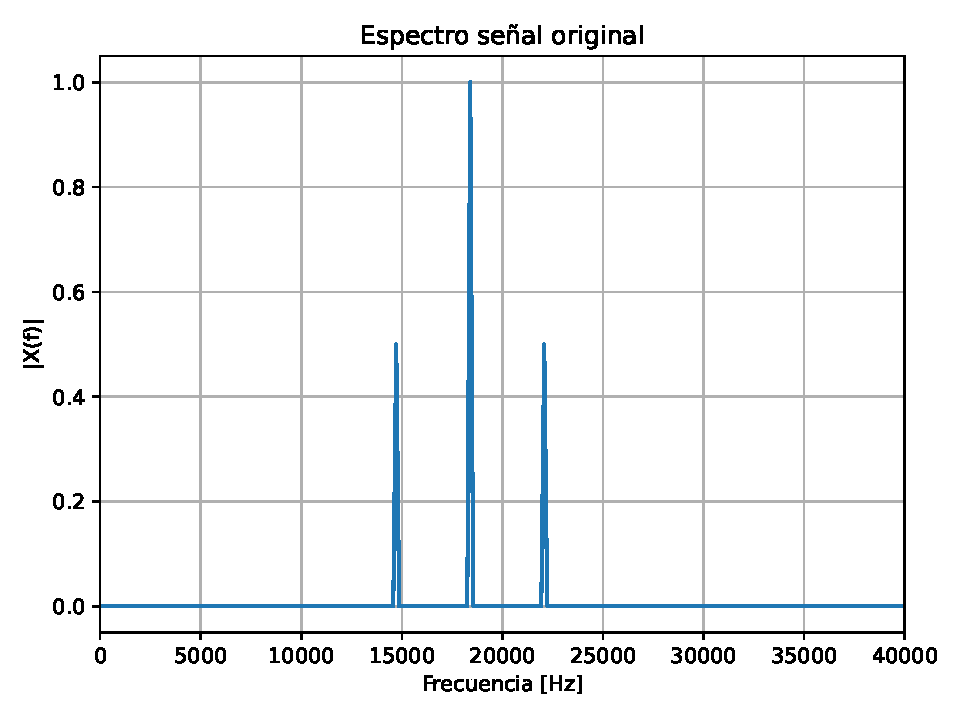
\includegraphics[width=\textwidth]{Imagenes/6_Mustreo_inst/espectro_original.pdf}
        \caption{Señal original}
        \label{fig: 6_espectro origial}
    \end{subfigure}

    \vspace{0.5cm}

    % Fila inferior (dos imágenes)
    \begin{subfigure}{0.48\textwidth}
        \centering
        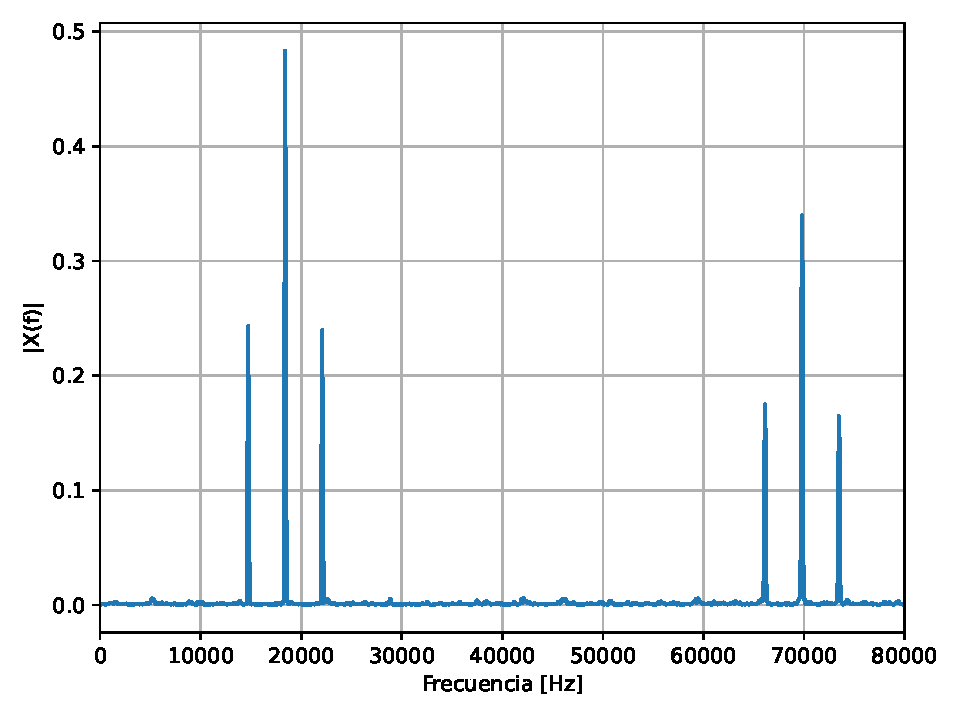
\includegraphics[width=\textwidth]{Imagenes/6_Mustreo_inst/espectro_pam.pdf}
        \caption{Señal muestreada.}
        \label{fig: 6_espectro_muestreada}
    \end{subfigure}
    \hfill
    \begin{subfigure}{0.48\textwidth}
        \centering
        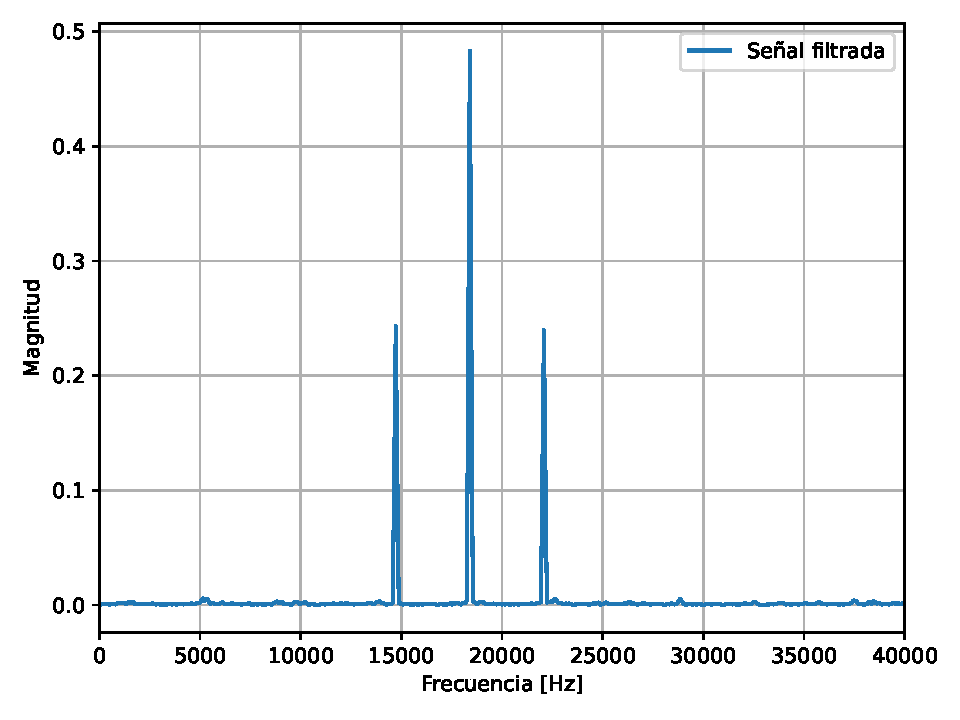
\includegraphics[width=\textwidth]{Imagenes/6_Mustreo_inst/espectro_filtrado.pdf}
        \caption{Señal muestreda + FR.}
        \label{fig: 6_muestreada_FR}
    \end{subfigure}

    \caption{Espectros teóricos.}
    \label{fig: 6_espectos teoricos}
\end{figure}

\noindent De este modo las simulaciones concuerdan con la expectativa teórica. Si se realizan las mediciones en la placa empíricamente:

\begin{figure}[H]
    \centering
    \begin{subfigure}{0.48\textwidth}
        \centering
        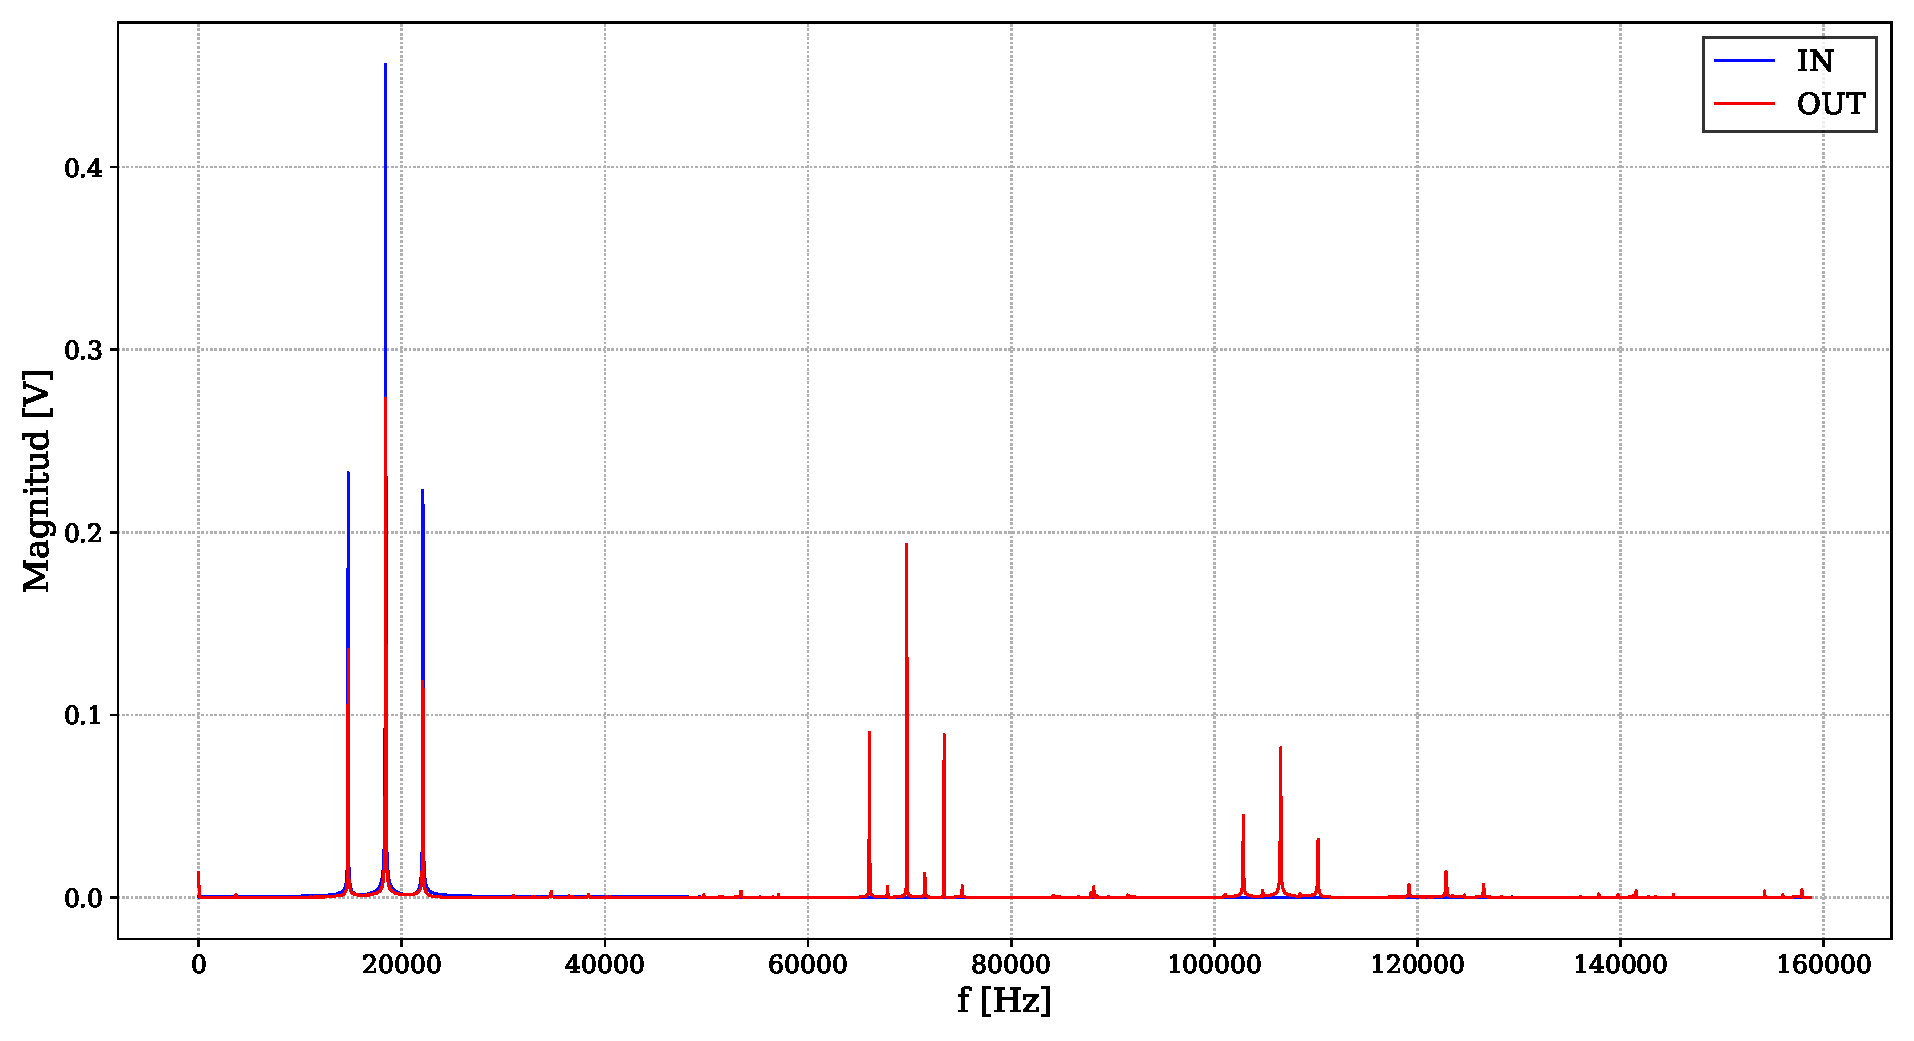
\includegraphics[width=\textwidth]{Imagenes/6_Mustreo_inst/FFFT_88_2_fs_9_2_fin_NO_FR}
        \caption{Sin FR.}
    \end{subfigure}
    \hfill
    \begin{subfigure}{0.48\textwidth}
        \centering
        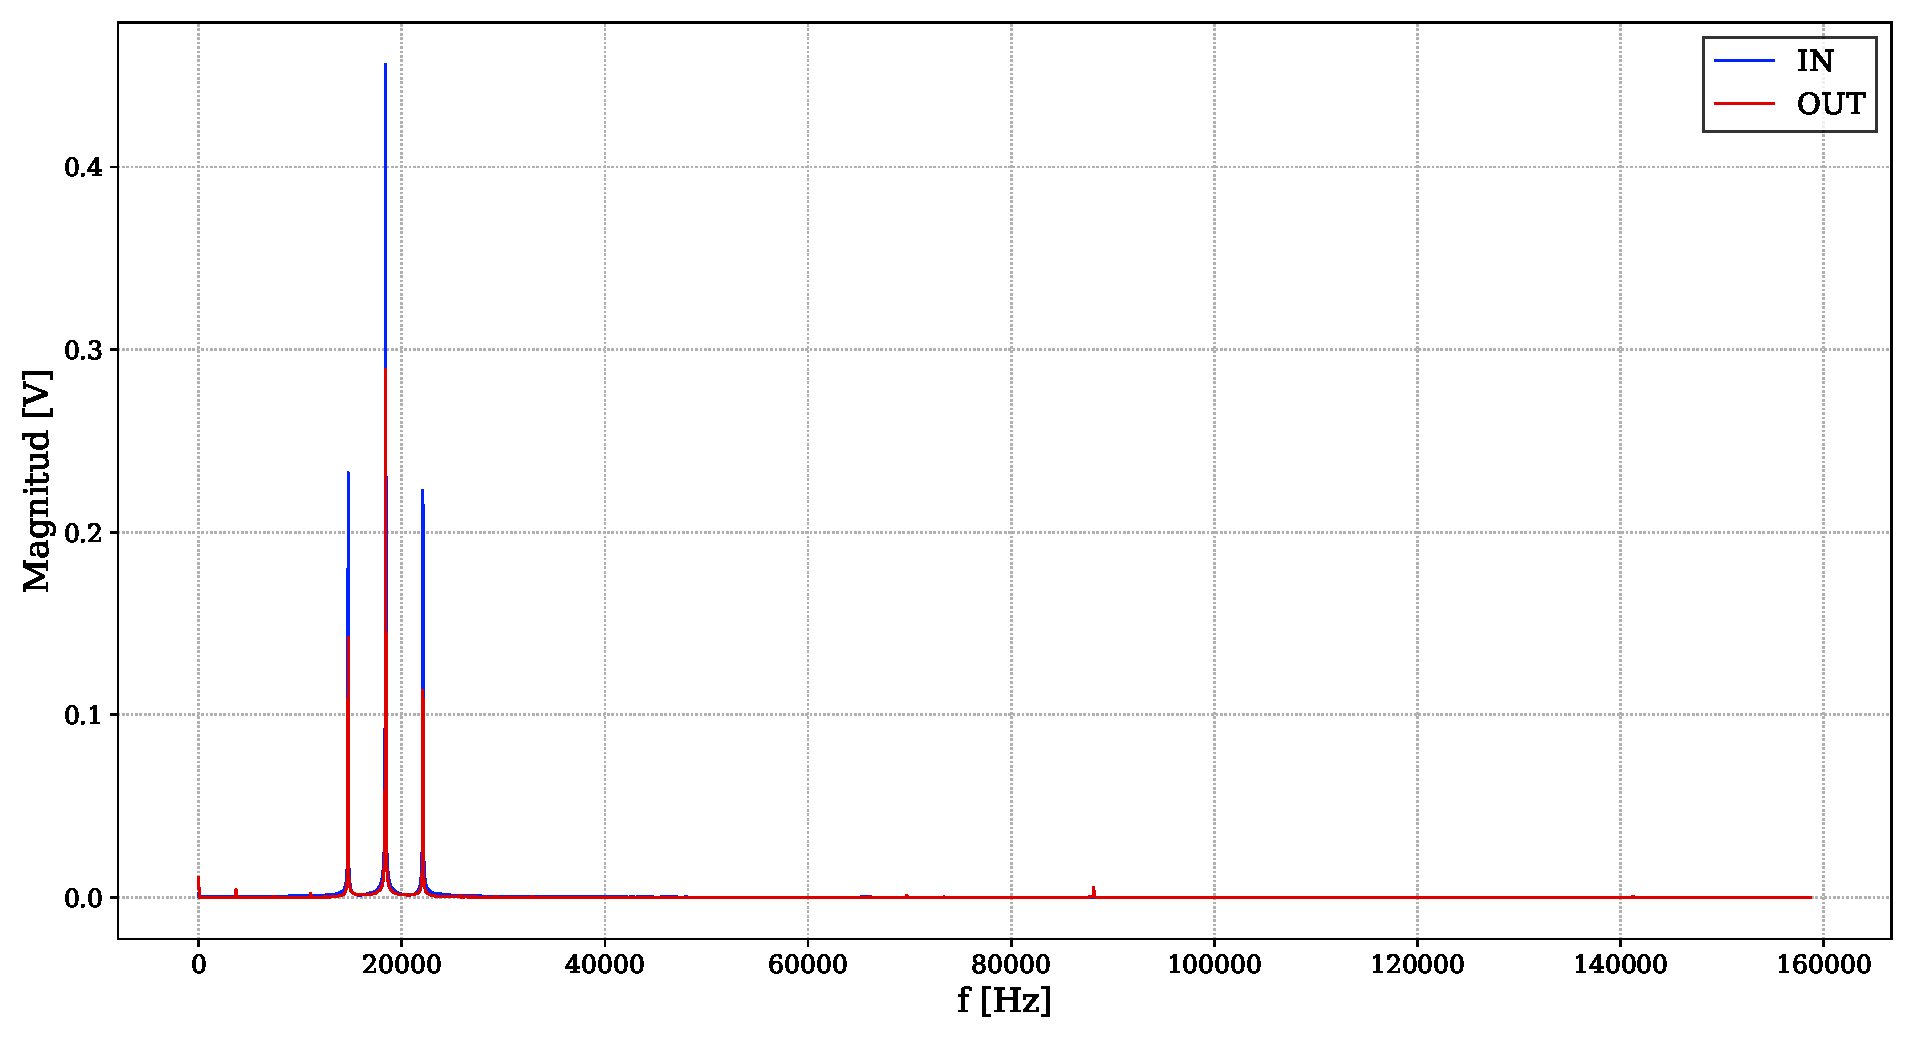
\includegraphics[width=\textwidth]{Imagenes/6_Mustreo_inst/FFFT_88_2_fs_9_2_fin_FR}
        \caption{Con FR.}
    \end{subfigure}
    \caption{Mediciones realizadas.}
\end{figure}

\noindent También se puede aprovechar la oportunidad de este caso límite para verificar que de haber tomado $f_s = 2 \cdot f_p$ se dispondría de un problema de alias:

\begin{figure}[H]
    \centering
    \begin{subfigure}{0.48\textwidth}
        \centering
        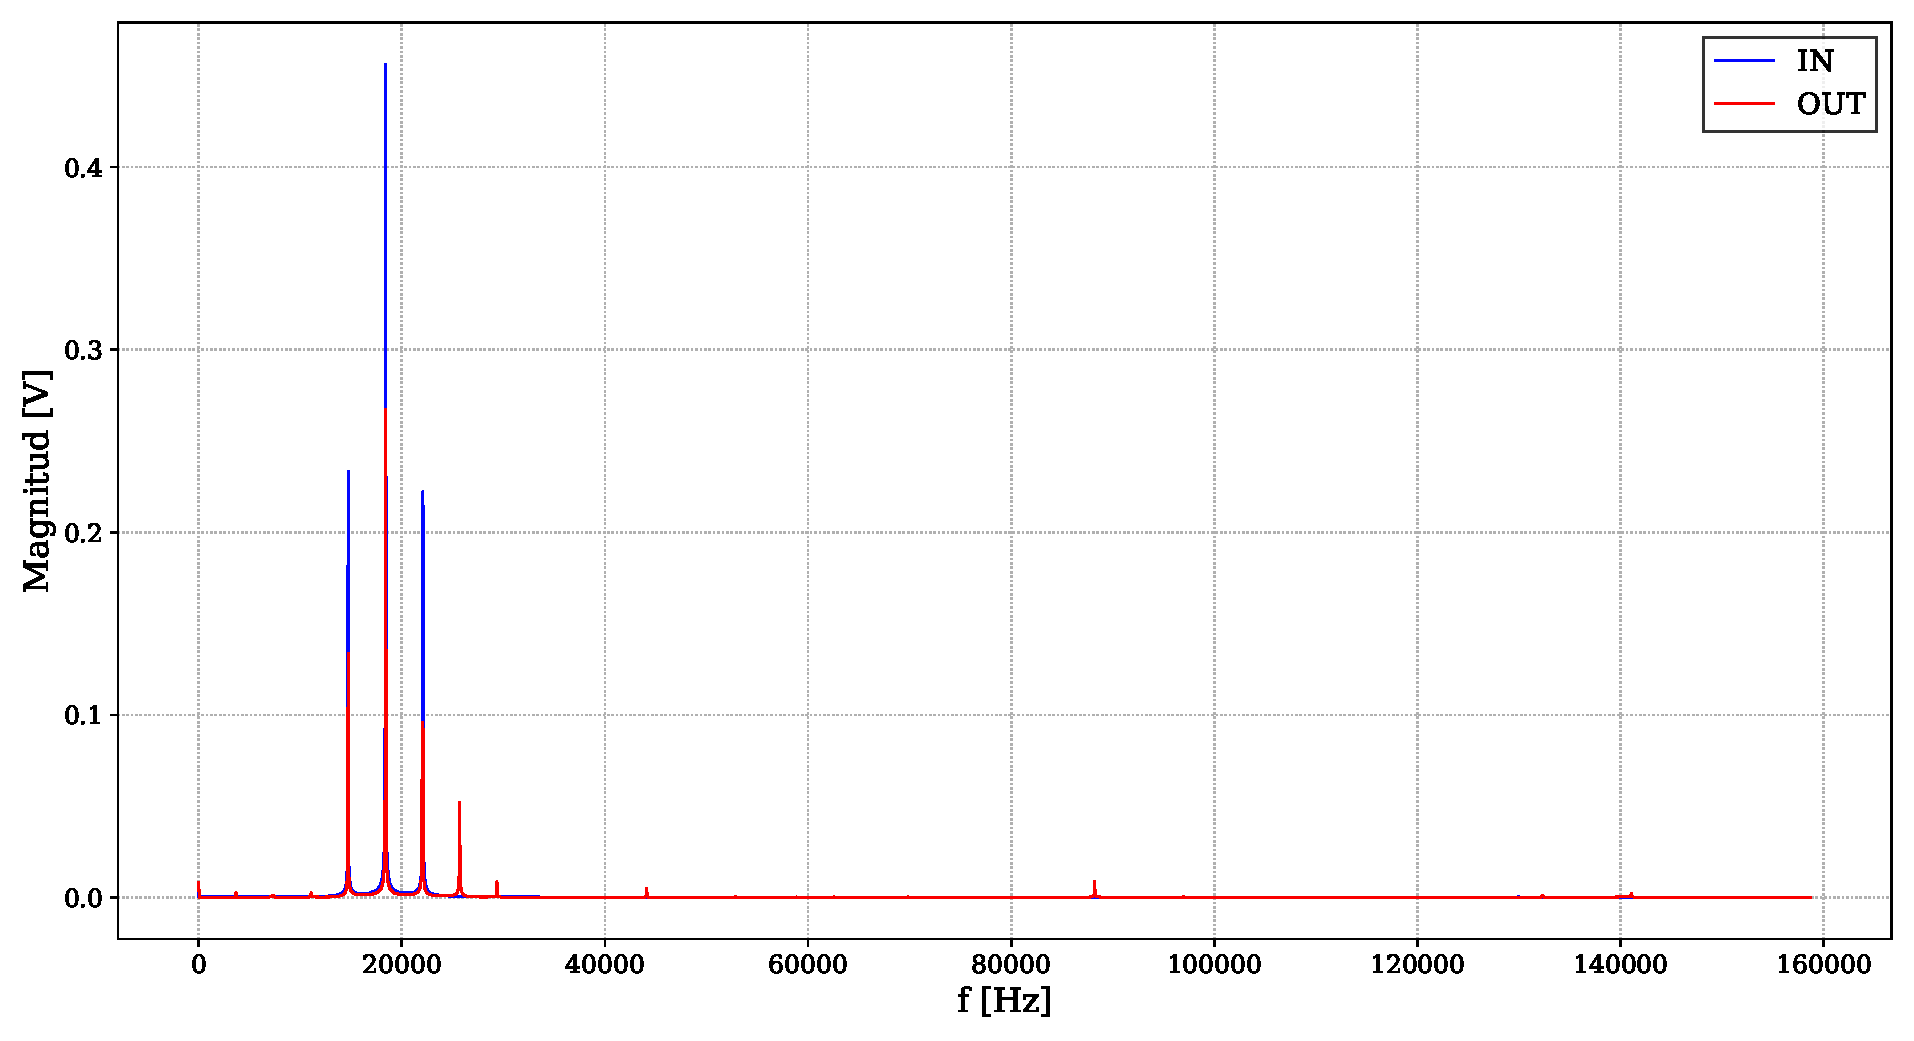
\includegraphics[width=\textwidth]{Imagenes/6_Mustreo_inst/FFFT_44_1_fs_9_2_fin_FR.pdf}
        \caption{Sin FR.}
    \end{subfigure}
    \hfill
    \begin{subfigure}{0.48\textwidth}
        \centering
        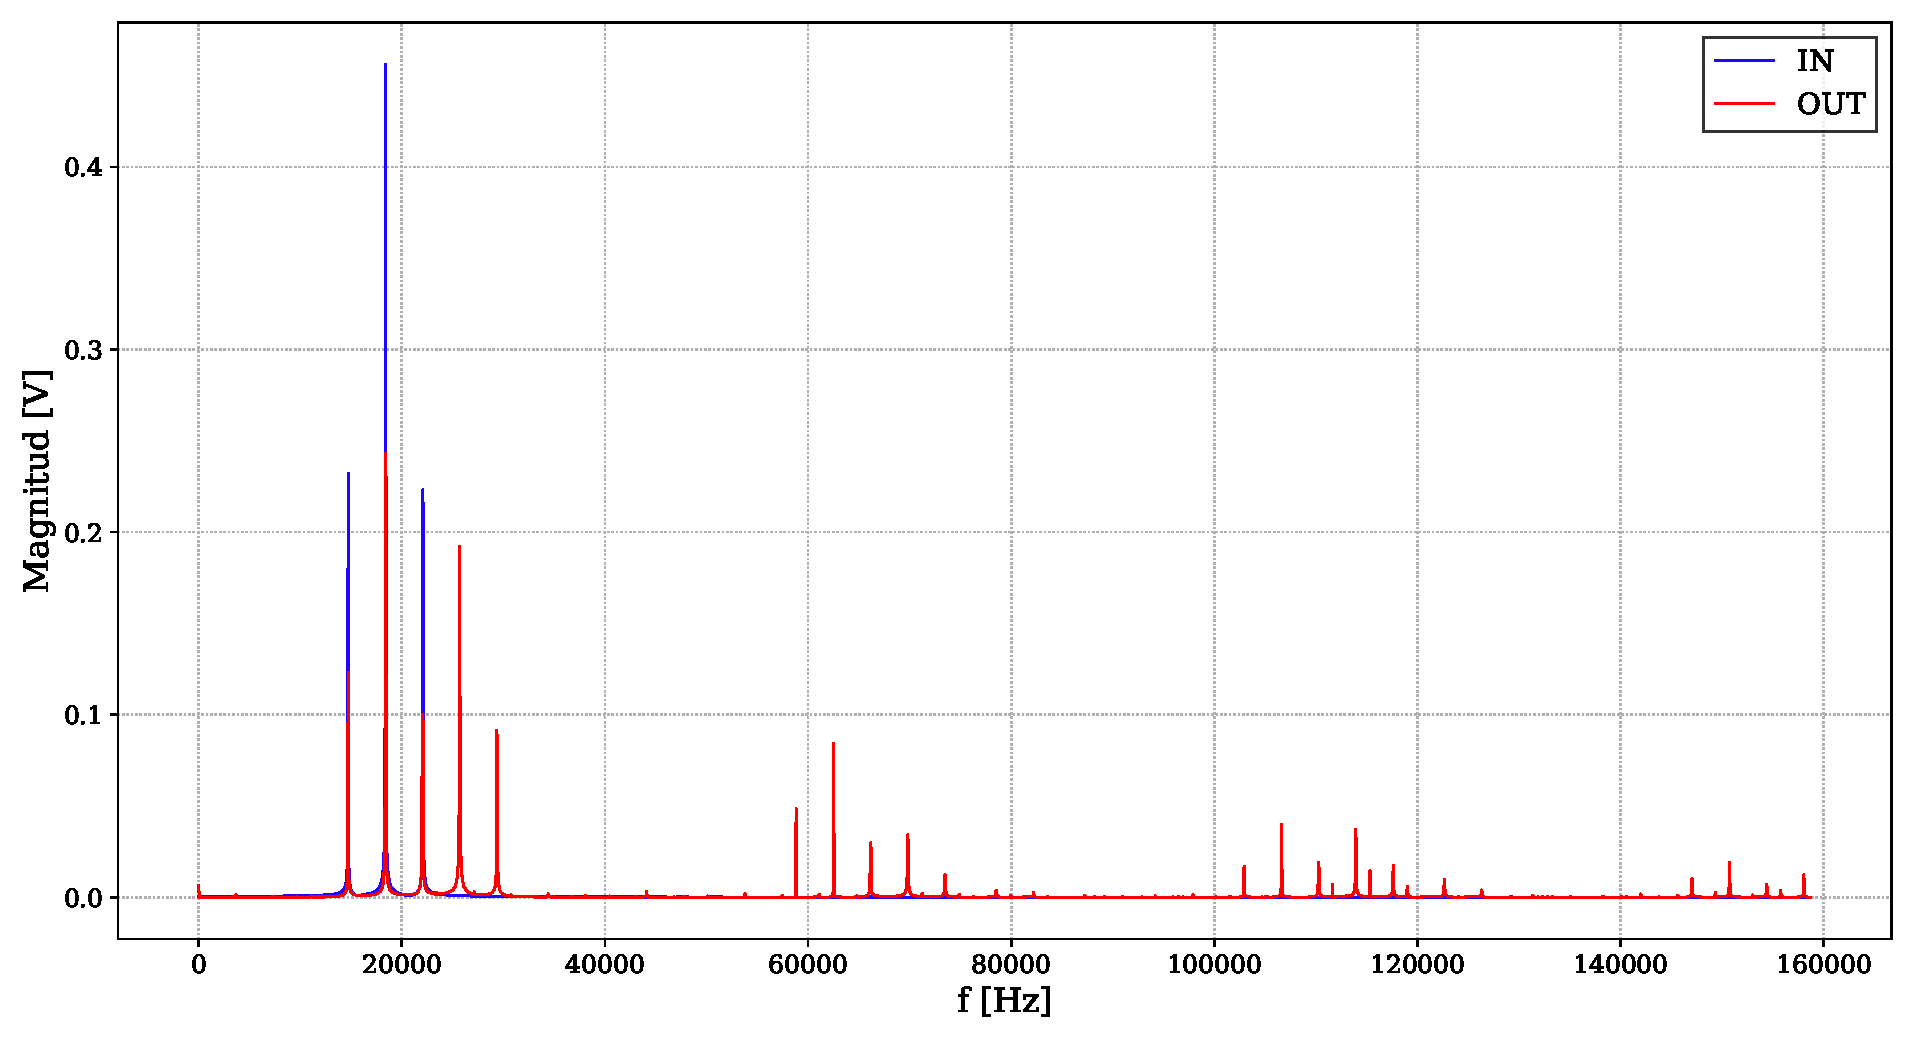
\includegraphics[width=\textwidth]{Imagenes/6_Mustreo_inst/FFFT_44_1_fs_9_2_fin_NO_FR.pdf}
        \caption{Con FR.}
    \end{subfigure}
    \caption{Mediciones realizadas con $f_s = 44.1khZ$.}
\end{figure}

